\documentclass[10.5pt,a4paper]{article}
\usepackage[margin=2.1cm]{geometry}
\usepackage[T1]{fontenc}
\usepackage{lmodern}
\usepackage{microtype}
\usepackage{booktabs}
\usepackage{tabularx}
\usepackage{xcolor}
\usepackage{tikz}
\usetikzlibrary{arrows.meta,positioning,shapes.geometric}
\usepackage[hidelinks]{hyperref}

\definecolor{accent}{HTML}{1F5FA8}
\definecolor{soft}{HTML}{EAF1FA}
\definecolor{good}{HTML}{1E7B4A}
\makeatletter
\renewcommand\section{\@startsection{section}{1}{\z@}{-2.2ex plus -1ex minus -.2ex}{1.0ex plus .2ex}{\large\bfseries\color{accent}}}
\renewcommand\subsection{\@startsection{subsection}{2}{\z@}{-1.6ex plus -.5ex minus -.2ex}{0.6ex plus .2ex}{\normalsize\bfseries}}
\makeatother
\let\olditemize\itemize
\renewcommand\itemize{\olditemize\setlength{\itemsep}{1pt}\setlength{\topsep}{2pt}\setlength{\parskip}{0pt}}
\setlength{\parskip}{3pt}
\setlength{\parindent}{0pt}
\newcommand{\hl}[1]{\textbf{\color{accent}#1}}

\begin{document}

{\LARGE\bfseries Delhi Bus Journey Planner}\\[2pt]
{\large A Google-Maps-like travel-time API built from bus GPS data}\\[4pt]
{\small Transport Stack Hackathon 2026 \quad$\cdot$\quad Data: DTC bus GPS, October 2026 \quad$\cdot$\quad 24 November 2026}

\vspace{6pt}
\noindent\colorbox{soft}{\parbox{\dimexpr\textwidth-2\fboxsep}{\small
\textbf{In one paragraph.} We turned 124 GB of raw bus GPS pings into a \emph{traffic model}: how long each stretch of road between two bus stops takes, by hour of day and weekday/weekend. A journey planner uses it to answer ``how do I get from A to B by bus, and how long will it take?''. On 600{,}000 rides from a held-out week, the final model (lookup table + an \textbf{XGBoost} correction trained on the GPU) is off by a median of \hl{12.3\%}, against \hl{32.5\%} for the official timetable. On popular passenger trips it is \hl{6.7\%} off, and closer to actual bus times than \hl{Google Maps} (9.6\% vs 16.3\%). A live layer cuts the error in ``when is my next bus?'' from about 8.5 minutes to \hl{under 2 minutes}.}}

%======================================================================
\section{Problem statement}

Delhi's DTC buses report their position every $\sim$10 seconds. Together they sample traffic across the whole road network, all day. The challenge:

\begin{itemize}
  \item \textbf{Build a traffic model} from historical (and real-time) bus location data.
  \item \textbf{Integrate it with a journey planner}: an API that takes two locations and returns plausible bus journey options with estimated travel times.
  \item \textbf{Be right:} estimates should match actual travel times for sample trips and compare well with Google Maps.
\end{itemize}

\textbf{Why it is hard.} The published timetable is a poor guide: buses run slower in rush hour and faster at night, and they bunch. The raw feed is noisy, with duplicate pings, GPS jumps, gaps, buses parked at depots, and trips tagged with the wrong direction. A journey also has more than a ride: walking to the stop, waiting, transferring and walking at the end.

%======================================================================
\section{What the data looks like}

\begin{center}\small
\begin{tabularx}{\textwidth}{@{}l X r@{}}
\toprule
\textbf{Dataset} & \textbf{Contents} & \textbf{Size} \\
\midrule
Bus GPS (31 daily SQLite files) & One row per ping: bus number, latitude/longitude, speed, route id, trip id, timestamp. About \textbf{29 M pings/day}, $\sim$6{,}000 buses, $\sim$2{,}100 routes, $\sim$81{,}000 trips/day. & 124 GB \\
Static GTFS (timetable) & 6{,}862 stops, 2{,}573 routes, 80{,}000 scheduled trips, route shapes (polylines), stop sequences. & 170 MB \\
E-ticketing (ONDC) & 2.56 M tickets: route, boarding stop, alighting stop, time, fare. Shows where people actually travel. & 290 MB \\
\bottomrule
\end{tabularx}
\end{center}

\textbf{A few observations shaped the design:}
\begin{itemize}
  \item The GPS \texttt{route\_id} matches the timetable's routes for \textbf{99\%} of routes (2{,}105 of 2{,}119), so every ping can be placed on a known route shape with known stops.
  \item Pings arrive every $\sim$10 s. About 12\% have speed 0, mostly buses idling at terminals.
  \item About 17\% of trips are tagged with the wrong direction's route (``UP'' instead of ``DOWN'').
  \item Ticket demand peaks at \textbf{09:00} and \textbf{18:00}. Ticket stop names are short (``Ashram'') while timetable names are compound (``Maharani Bagh / Ashram''), so names must be matched.
\end{itemize}

%======================================================================
\section{Our solution}

\begin{center}
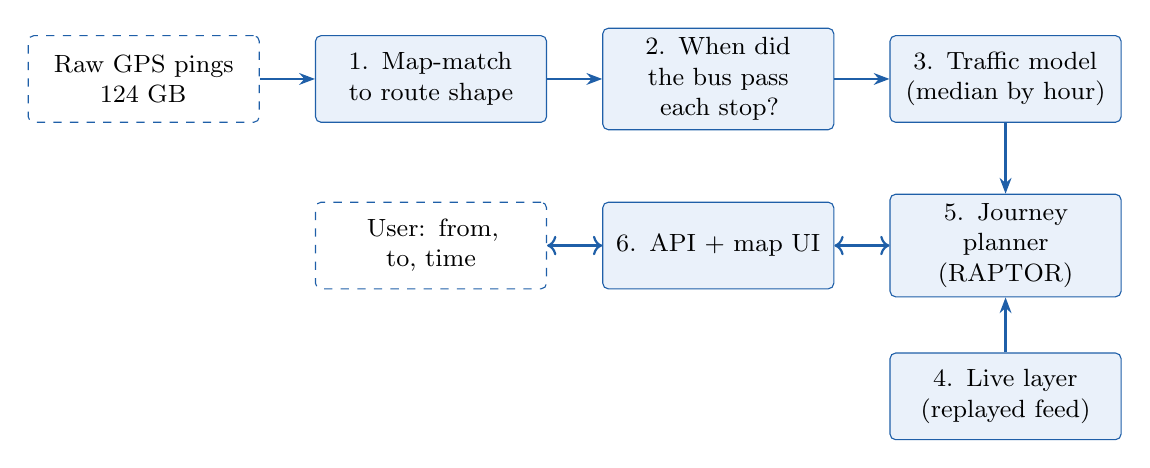
\begin{tikzpicture}[
  node distance=5mm and 7mm,
  box/.style={draw=accent, fill=soft, rounded corners=2pt, align=center, font=\small, minimum height=11mm, text width=27mm},
  data/.style={box, fill=white, dashed},
  arr/.style={-{Stealth[length=2mm]}, thick, accent}]
\node[data] (gps) {Raw GPS pings\\124 GB};
\node[box, right=of gps] (match) {1. Map-match to route shape};
\node[box, right=of match] (pass) {2. When did the bus pass each stop?};
\node[box, right=of pass] (agg) {3. Traffic model\\(median by hour)};
\node[box, below=9mm of agg] (plan) {5. Journey planner\\(RAPTOR)};
\node[box, left=of plan] (api) {6. API + map UI};
\node[box, below=7mm of plan] (live) {4. Live layer\\(replayed feed)};
\node[data, left=of api] (user) {User: from, to, time};
\draw[arr] (gps) -- (match); \draw[arr] (match) -- (pass); \draw[arr] (pass) -- (agg);
\draw[arr] (agg) -- (plan); \draw[arr] (live) -- (plan);
\draw[arr, <->] (plan) -- (api); \draw[arr, <->] (user) -- (api);
\end{tikzpicture}
\end{center}

\subsection*{Steps 1--2: From pings to ``stop passing'' times}
For each trip we project every ping onto the route's GTFS shape to get \emph{distance travelled along the route}. We remove noise: points over 150 m off the route, backward jumps and terminal dwell. We then interpolate the moment the bus passed each stop. Two consecutive passings give one observed \textbf{stop-to-stop travel time}. Across the month this gives \textbf{35 M stop passings} and \textbf{33 M segment observations}. Each day is processed in parallel on the data machine; only small summary tables leave it.

\subsection*{Step 3: The traffic model: deterministic, by design}
For every route segment (stop A $\rightarrow$ stop B), hour of day and day type (weekday/weekend), we store the median, mean and 85th-percentile travel time and the number of observations. Gaps are filled in this order:
\begin{center}\small
segment's own data $\rightarrow$ same stop pair on any route $\rightarrow$ timetable $\times$ fitted hour-of-day factor $\rightarrow$ distance / 15 km/h
\end{center}
\textbf{Waiting time} comes from the \emph{observed} gaps between consecutive buses at each stop (half the gap, capped), not from the timetable.

We chose a lookup model over ML first: it is fast to build, easy to explain (``the median of 1{,}000 real buses on this road at 9 am''), and the data covers \textbf{90.5\%} of all route segments. Sums of medians come out too short on long rides, because delays are skewed, so the planner uses medians for the first 10 minutes of a ride and means after that.

\subsection*{Step 3b: ML correction (final submission)}
An \textbf{XGBoost} model, trained on the GPU, adjusts each bus leg's lookup estimate using its length, number of stops, hour, day type, route speed, how variable the segments are, and how much of the leg had no data of its own. It was trained on days 1--18, tuned on days 19--24, refit on 1--24 and tested on 25--31. It helps most on \textbf{long rides} (over 1 h: 18.3\% $\rightarrow$ 14.0\% error).

\subsection*{Step 4: Real-time layer}
A held-out day (28 Oct) is replayed as if it were live. Every 15 s we compare the last 30 minutes of observed segment times with the historical value and get a \emph{live slow-down ratio} per segment, falling back to the 3$\times$3 km area and then the whole city. Live bus positions also give a \textbf{next-bus ETA} at each stop.

\subsection*{Step 5: Journey planner}
A frequency-based \textbf{RAPTOR} router: each round adds one bus leg, up to 3 transfers. It includes walking to and from stops within 800 m and transfers between stops within 400 m. Options are ranked with a 10-minute penalty per transfer, and the best direct bus is always shown. The API returns up to 3 options, each with its legs, routes, waits, a time range (typical to heavy traffic) and map polylines.

\subsection*{Step 6: API}
FastAPI: \texttt{GET /journey?from\_lat\&from\_lng\&to\_lat\&to\_lng\&depart[\&realtime=1]}, plus stop search and a Leaflet map page. Responses take \textbf{$\sim$100--400 ms}.

%======================================================================
\section{Results}

All evaluations use data the model has not seen: the model is built from \textbf{1--24 October} and tested on \textbf{25--31 October}.

\subsection*{4.1\; 600{,}000 held-out bus rides}
\begin{center}\small
\begin{tabular}{@{}lccc@{}}
\toprule
\textbf{Method} & \textbf{Median error} & \textbf{Within $\pm$20\%} & \textbf{Bias} \\
\midrule
Official GTFS timetable & 32.5\% & 32.6\% & --- \\
Sum of segment medians & 12.7\% & 67.8\% & $-120$ s \\
Lookup model (median$\rightarrow$mean blend) & 12.5\% & 68.3\% & $-74$ s \\
ML correction, LightGBM & 12.3\% & 68.9\% & $-71$ s \\
\textbf{Final: lookup + XGBoost (GPU)} & \textbf{12.3\%} & \textbf{69.0\%} & $-73$ s \\
\bottomrule
\end{tabular}
\end{center}
The final model is about \textbf{2.6$\times$ more accurate than the timetable}. On rides over 1 hour, XGBoost cuts the error from 18.3\% to 14.0\%. These are single random rides, which include day-to-day noise such as a breakdown or a jam on one day.

\subsection*{4.2\; Popular trips from ticketing data (60 pairs, actual rides 26--30 Oct)}
We picked 60 origin--destination pairs from real ticket demand: short, medium and long, across all parts of Delhi, at peak and off-peak, including transfers. All 60 got plausible answers. Median door-to-door speed is 11.5 km/h (13.0 at 9 am, 9.9 at 6:30 pm).
\begin{center}\small
\begin{tabular}{@{}lccc@{}}
\toprule
\textbf{Ride time vs actual} & \textbf{Median error} & \textbf{Within $\pm$20\%} & \textbf{Bias} \\
\midrule
GTFS timetable & 20.7\% & 49\% & $-12.4$\% \\
\textbf{Our planner} & \textbf{6.7\%} & \textbf{84\%} & $+2.0$\% \\
\bottomrule
\end{tabular}
\end{center}

\subsection*{4.3\; Comparison with Google Maps}
We collected Google Maps transit times for 30 pairs. On the 18 pairs where we also have actual GPS rides:
\begin{center}\small
\begin{tabular}{@{}lccc@{}}
\toprule
\textbf{Estimate vs actual bus ride} & \textbf{Median error} & \textbf{Within $\pm$20\%} & \textbf{Bias} \\
\midrule
GTFS timetable & 21.2\% & 44\% & $-16.9$\% \\
Google Maps & 16.3\% & 56\% & $-10.6$\% \\
\textbf{Our planner} & \textbf{9.6\%} & \textbf{89\%} & $-2.8$\% \\
\bottomrule
\end{tabular}
\end{center}
\textbf{Google Maps underestimates Delhi bus times}, most of all in the evening peak. Example: Mahipal Pur $\rightarrow$ Andheria More at 18:30. Google says 24 min, we say 36 min, and buses actually took 42 min.

\subsection*{4.4\; Real-time layer (replayed day, $\sim$130{,}000 rides)}
\begin{center}\small
\begin{tabular}{@{}lcc@{}}
\toprule
 & \textbf{Historical only} & \textbf{+ Live} \\
\midrule
Ride time error (boarding in next 30 min) & 11.7\% & 11.7\% (bias $-6.3\% \rightarrow -1.6\%$) \\
\textbf{Next-bus wait error} & 503 s ($\approx$ 8.4 min) & \textbf{107 s} ($<$ 2 min) \\
Next-bus predictions within $\pm$2 min & 14\% & \textbf{53\%} \\
\bottomrule
\end{tabular}
\end{center}
Live data barely changes ride times, but it is very good for \emph{when the next bus comes}, which is the biggest uncertainty for a rider.

\subsection*{4.5\; What the data says about Delhi traffic}
\begin{center}
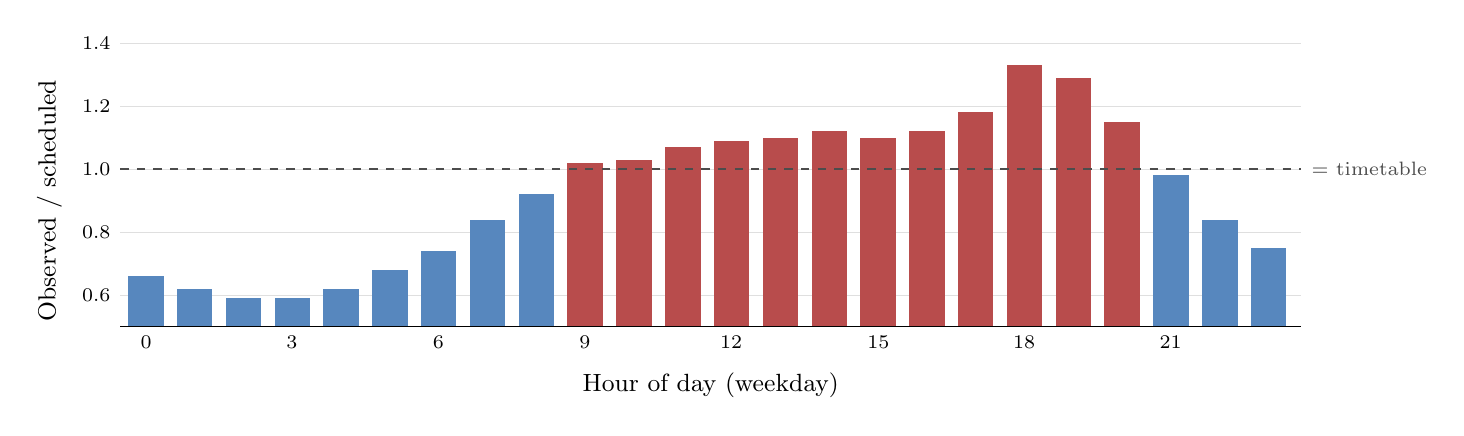
\begin{tikzpicture}
\draw[gray!25] (-0.1,0.40) -- (14.9,0.40); \node[font=\scriptsize,left] at (-0.1,0.40) {0.6};
\draw[gray!25] (-0.1,1.20) -- (14.9,1.20); \node[font=\scriptsize,left] at (-0.1,1.20) {0.8};
\draw[gray!25] (-0.1,2.00) -- (14.9,2.00); \node[font=\scriptsize,left] at (-0.1,2.00) {1.0};
\draw[gray!25] (-0.1,2.80) -- (14.9,2.80); \node[font=\scriptsize,left] at (-0.1,2.80) {1.2};
\draw[gray!25] (-0.1,3.60) -- (14.9,3.60); \node[font=\scriptsize,left] at (-0.1,3.60) {1.4};
\fill[accent!75] (0.00,0) rectangle (0.45,0.64);
\fill[accent!75] (0.62,0) rectangle (1.07,0.48);
\fill[accent!75] (1.24,0) rectangle (1.69,0.36);
\fill[accent!75] (1.86,0) rectangle (2.31,0.36);
\fill[accent!75] (2.48,0) rectangle (2.93,0.48);
\fill[accent!75] (3.10,0) rectangle (3.55,0.72);
\fill[accent!75] (3.72,0) rectangle (4.17,0.96);
\fill[accent!75] (4.34,0) rectangle (4.79,1.36);
\fill[accent!75] (4.96,0) rectangle (5.41,1.68);
\fill[red!60!black!70] (5.58,0) rectangle (6.03,2.08);
\fill[red!60!black!70] (6.20,0) rectangle (6.65,2.12);
\fill[red!60!black!70] (6.82,0) rectangle (7.27,2.28);
\fill[red!60!black!70] (7.44,0) rectangle (7.89,2.36);
\fill[red!60!black!70] (8.06,0) rectangle (8.51,2.40);
\fill[red!60!black!70] (8.68,0) rectangle (9.13,2.48);
\fill[red!60!black!70] (9.30,0) rectangle (9.75,2.40);
\fill[red!60!black!70] (9.92,0) rectangle (10.37,2.48);
\fill[red!60!black!70] (10.54,0) rectangle (10.99,2.72);
\fill[red!60!black!70] (11.16,0) rectangle (11.61,3.32);
\fill[red!60!black!70] (11.78,0) rectangle (12.23,3.16);
\fill[red!60!black!70] (12.40,0) rectangle (12.85,2.60);
\fill[accent!75] (13.02,0) rectangle (13.47,1.92);
\fill[accent!75] (13.64,0) rectangle (14.09,1.36);
\fill[accent!75] (14.26,0) rectangle (14.71,1.00);
\draw[dashed, thick, black!70] (-0.1,2) -- (14.9,2) node[right,font=\scriptsize]{= timetable};
\draw (-0.1,0) -- (14.9,0);
\node[font=\scriptsize,below] at (0.23,0) {0};
\node[font=\scriptsize,below] at (2.08,0) {3};
\node[font=\scriptsize,below] at (3.94,0) {6};
\node[font=\scriptsize,below] at (5.80,0) {9};
\node[font=\scriptsize,below] at (7.66,0) {12};
\node[font=\scriptsize,below] at (9.53,0) {15};
\node[font=\scriptsize,below] at (11.38,0) {18};
\node[font=\scriptsize,below] at (13.24,0) {21};
\node[font=\small] at (7.4,-0.75) {Hour of day (weekday)};
\node[font=\small,rotate=90] at (-1.0,1.6) {Observed / scheduled};
\end{tikzpicture}
\end{center}
{\small Buses take about \textbf{40\% less} than the timetable at night and \textbf{33\% more} at 6 pm. Average network speed is $\sim$32 km/h at 3 am, 21 km/h at 8 am, 18 km/h midday and 15 km/h at 6--7 pm.}

%======================================================================
\section{Miscellaneous}

\subsection*{Did ML help?}
Yes, a little. Overall it improves on the lookup model by about 0.2--0.4 points (12.69\% $\rightarrow$ 12.28\% median error on 600 k test rides). Its real value is on \textbf{long rides} (18.3\% $\rightarrow$ 14.0\%), on routes with little data, and in the evening peak. The final XGBoost model is used by the API by default. A stronger model is unlikely to help much more: the remaining error is mostly day-to-day and bus-to-bus variation, which only live data can address.

\subsection*{Limitations}
\begin{itemize}
  \item Rides over an hour remain the hardest (14\% median error, still slightly under-predicted): long stalls were filtered out as noise during cleaning.
  \item Only 68\% of GPS trips are usable. Wrong-direction tags and loop routes lose the rest.
  \item One stop pattern per route, so short-turn variants are ignored. Walking is straight-line $\times$ 1.3, with no street network.
  \item ``Real-time'' is a replay of a past day. A live feed client is a small addition.
  \item The Google comparison is small (30 pairs) and from a different week. Google cannot be queried for past dates.
\end{itemize}

\subsection*{Next steps}
Keep stall segments for long rides; tag trip direction by matching to both UP and DOWN routes; support several stop patterns per route; connect a live GTFS-RT feed; add Metro for multimodal trips; deploy publicly (Docker container).

\subsection*{How it was built}
Two people plus a team of AI coding agents working in parallel: data/model, planner/API, evaluation, real-time and ML. Heavy processing ran on a 20-core Windows workstation next to the data, so raw data never left it. All 31 days were processed in $\sim$47 min. Code, documentation and a decision log live in one git repository.

%======================================================================
\clearpage
\appendix
\renewcommand{\thesection}{\Alph{section}}
{\LARGE\bfseries\color{accent} Technical appendix}\\[2pt]
{\small Everything below is detail for readers who want to check or reproduce the work. Paths refer to the git repository \texttt{E:\textbackslash hackathon-project}.}

\section{Data processing: from pings to stop passings}
\textbf{Route patterns.} For each GTFS \texttt{route\_id} we take the most common stop sequence among its scheduled trips (\texttt{route\_patterns.csv}, 2{,}574 routes, 82{,}000 rows) and its shape polyline. We compute each stop's distance along the shape (\texttt{model/scripts/build\_patterns.py}).

\textbf{Per-trip processing} (\texttt{model/scripts/process\_day.py}, one process per day):
\begin{itemize}
  \item Read the day's \texttt{vehicle\_feed} in one sequential scan (about 2 min of the run). Group by \texttt{trip\_id}, sort by timestamp, drop duplicate pings.
  \item Project each ping onto the route shape (nearest segment of the polyline) to get distance along the route and the offset from the shape.
  \item Reject pings more than 150 m from the shape. Enforce near-monotonic progress (small backward jitter tolerated, big jumps dropped). Trim dwell at the start and end terminals.
  \item Interpolate the time at which the bus crossed each stop's distance. Consecutive crossings give a segment time, measured passing to passing, so dwell at stops is included.
  \item Sanity filters: drop segments with implied speed over 70 km/h, ping gaps over 300 s, or segment times over 30 min.
\end{itemize}

\textbf{Trip outcomes} (1 Oct, 80{,}650 trips): usable 57{,}945 (72\%); not moving along the route (\emph{no\_progress}) 6{,}470; too short 6{,}009; off the shape 5{,}926; filtered 2{,}188; too few stops 2{,}069; route missing from GTFS 43. Over the month about 68\% of trips are usable, giving $\sim$1.5 M stop passings per day (\texttt{E:\textbackslash hackathon-work\textbackslash pass\textbackslash pass\_DD.npz}, $\sim$40 MB/day).

\textbf{Wrong-direction trips.} In a sample, $\sim$17\% of trips fit their labelled route poorly, often because they run the paired UP/DOWN route. Also trying the paired route (\texttt{USE\_PAIR=1}) recovered only $\sim$5\% more trips at 2$\times$ the CPU, so it is off for the main run.

\textbf{Compute.} Windows workstation, 20 logical CPUs, 64 GB RAM. One day takes $\sim$5 min alone and 15--20 min when 10--18 days run in parallel (disk-bound). All 31 days took $\sim$47 min; aggregation takes $\sim$3 min.

\section{The traffic model}
\textbf{Tables} (built from 1--24 Oct by \texttt{model/scripts/aggregate.py}):
\begin{center}\small
\begin{tabularx}{\textwidth}{@{}l r X@{}}
\toprule
\textbf{File} & \textbf{Rows} & \textbf{Columns} \\
\midrule
\texttt{segment\_times.csv} & 1.80 M & route\_id, from\_stop, to\_stop, hour (IST, of entering the segment), daytype (weekday/weekend), median\_s, p85\_s, n, mean\_s \\
\texttt{stop\_headways.csv} & 1.61 M & stop\_id, route\_id, hour, daytype, median\_headway\_s, n \\
\texttt{holdout\_trips.csv} & 20 k & route\_id, board\_stop, alight\_stop, depart\_ts\_ist, actual\_s (random rides from 25--31 Oct) \\
\bottomrule
\end{tabularx}
\end{center}
\textbf{Coverage.} 72{,}002 of 79{,}592 GTFS route segments (90.5\%) have observations, and 70{,}788 have at least 5. 2{,}203 of 2{,}574 routes are covered. 33.4 M segment observations in total.

\textbf{Lookup chain} (\texttt{planner/ttmodel.py}); each cell is [segment, daytype, hour]:
\begin{enumerate}\itemsep0pt
  \item observed median for the route segment, if $n \ge 3$;
  \item observed value for the same stop pair on any route ($n$-weighted);
  \item GTFS scheduled time $\times$ fitted hour-of-day factor $\times$ that segment's own observed/scheduled ratio;
  \item distance / 15 km/h.
\end{enumerate}
Weekend cells with no data borrow weekday factors. In the dense tables, 1.50 M cells are filled from the route segment, 1.52 M from the stop pair, 0.69 M from schedule $\times$ segment ratio, and 0.10 M from schedule $\times$ hour factor.

\textbf{Median vs mean.} Segment times are right-skewed. Summing medians under-predicts long rides (bias $-1148$ s on rides over 1 h); summing means over-predicts short ones. The planner uses medians for the first 600 s of a ride and means after that (\texttt{SEG\_MODE=blend}, \texttt{BLEND\_S=600}):
\begin{center}\small
\begin{tabular}{@{}lcccc@{}}
\toprule
\textbf{Variant (20 k held-out rides)} & \textbf{Median error} & \textbf{Within $\pm$20\%} & \textbf{Median bias} & \textbf{Rides $>$1 h: error / bias} \\
\midrule
Median only & 12.8\% & 67.8\% & $-19$ s & 17.5\% / $-819$ s \\
Mean only & 13.7\% & 64.9\% & $+8$ s & 13.3\% / $-411$ s \\
Blend, switch at 10 min (default) & 12.6\% & 68.4\% & $-11$ s & 14.0\% / $-474$ s \\
GTFS schedule & 32.5\% & 32.6\% & $+63$ s & --- \\
\bottomrule
\end{tabular}
\end{center}

\textbf{Waiting.} Wait = min(headway/2, 20 min), using the observed median headway of that route at that stop and hour. If there is none, GTFS trips per hour are used; if the route has no service in that hour, the wait is 45 min. The 85th-percentile time band also widens with wait spread.

\section{Final ML model (XGBoost)}
\textbf{Ride-level dataset} (\texttt{model/v3/scripts/build\_rides.py}). Rides are random (route, board stop, alight stop, departure) samples from the per-day stop passings. To avoid leakage, each training ride's features come from lookup tables built on \emph{other} days: days 1--24 are split into 4 folds of 6 days, each with tables from the remaining 18 days. Test rides (days 25--31) use the 1--24 tables, which is exactly what the planner serves. In total: 1.2 M training rides and 600 k test rides.

\textbf{Target and features.} Target: $\log(\mathrm{actual} / \sum \mathrm{segment\ medians})$; prediction = base $\times\, e^{\hat y}$, clipped to [0.5, 2.5]. Features (20): log base time, mean/median skew, number of stops, log distance, base speed, hour (fractional), weekend, route length, route stop count, route speed, log route observations, route coverage, route skew, board position on the route, board and alight coordinates, share of segments with little data, and mean log observation count.

\textbf{Split and tuning} (\texttt{model/v3/scripts/xgb\_final.py}). Train on days 1--18. Validate on days 19--24, choosing among 3 configurations (depth 7--10, learning rate 0.03--0.05) and the number of trees by validation median error, checked every 100 trees. Refit on days 1--24. Test once on 25--31. Chosen: depth 10, learning rate 0.03, min child weight 50, 100 trees, absolute-error objective, \texttt{xgboost 2.1.4} on an RTX 3090 (84 s for the whole script).

\begin{center}\small
\begin{tabular}{@{}lcccc@{}}
\toprule
\textbf{Test rides (25--31 Oct, $n$=600 k)} & \textbf{Median error} & \textbf{Mean error} & \textbf{Within $\pm$20\%} & \textbf{Mean bias} \\
\midrule
Sum of segment medians & 12.69\% & 18.48\% & 67.8\% & $-120$ s \\
Sum of segment means & 13.58\% & 20.89\% & 64.9\% & $-34$ s \\
Median$\rightarrow$mean blend & 12.45\% & 18.33\% & 68.3\% & $-74$ s \\
Calibration by ride length & 12.43\% & 18.42\% & 68.4\% & $-76$ s \\
LightGBM (absolute error) & 12.32\% & 17.91\% & 68.9\% & $-71$ s \\
\textbf{XGBoost final} & \textbf{12.28\%} & \textbf{17.94\%} & \textbf{69.0\%} & $-73$ s \\
\bottomrule
\end{tabular}
\hspace{4mm}
\end{center}
\begin{center}\small
\begin{tabular}{@{}lcc@{}}
\toprule
\textbf{Ride length} & \textbf{Sum of medians} & \textbf{XGBoost final} \\
\midrule
$<$ 10 min & 13.18\% & 13.39\% \\
10--30 min & 11.36\% & 11.02\% \\
30--60 min & 12.97\% & 11.23\% \\
$>$ 60 min & 18.33\% & \textbf{13.99\%} \\
\bottomrule
\end{tabular}
\end{center}
\textbf{What it learns} (share of gain): number of stops 15.8\%, segment skew 14.7\%, share of sparse segments 13.7\%, hour 7.1\%, weekend 6.0\%, route speed 4.0\%, base speed 3.9\%. Adding day of week overfit (only 3--4 of each weekday in training), so it is excluded.

\textbf{Serving.} \texttt{model/v3/predict.py} recomputes the base from its own copy of the 1--24 Oct tables (\texttt{v3\_lookup.npz}), so serving matches training. The router calls it for each bus leg of the chosen options and scales the 85th-percentile band by the same ratio. \texttt{V3\_MODE=xgb} (default), \texttt{lgbm}, \texttt{calib} or \texttt{off}.

\section{Journey planner}
\textbf{Network} (\texttt{planner/preprocess.py}, $\sim$17 s): one stop pattern per route, shape with stop positions, scheduled segment times and trips per hour, and 17{,}865 footpaths between stops within 400 m (walking speed 1.2 m/s, detour factor 1.3).

\textbf{Routing} (\texttt{planner/router.py}). Frequency-based RAPTOR: round $k$ adds the $k$-th bus leg (at most 4 legs, so 3 transfers), and ride times depend on the hour. Access and egress use stops within 800 m, widening to 1.5 km and then 2.5 km if none are found. Candidates come from a time-optimal run, a walk-averse run (walking cost $\times$3) and up to 3 diversity runs that ban routes already found. Each candidate is re-timed segment by segment as the hour changes. Junk is removed: re-boarding the same route, 1-stop hops, and transfers with a ride under 4 min.

\textbf{Ranking.} Generalised cost = time + 10 min per transfer + extra weight on waiting and walking. The best direct bus is always included when it is within 20\% of the fastest. Labels: recommended, fastest, direct, fewest transfers, least walking. This cut ``transfer recommended when a direct bus exists'' on the test pairs from 11 to 5.

\section{Real-time layer}
\textbf{Replay} (\texttt{realtime/}). 28 Oct, 06:00--22:00, one ping per vehicle every $\ge$30 s: 6.7 M rows, 6{,}308 vehicles, 73 MB (\texttt{E:\textbackslash hackathon-work\textbackslash realtime\textbackslash replay\_28.npz}). \texttt{ReplayFeed} runs a simulated clock with a speed multiplier.

\textbf{Live ratio.} Pings are projected onto route shapes, also trying the paired UP/DOWN route, to detect stop passings in the last 30 min. The ratio observed / historical is pooled segment $\rightarrow$ 3$\times$3 km cell $\rightarrow$ city $\rightarrow$ 1.0, with each level shrunk toward the next when it has few observations, and clipped to [0.6, 2.5]. It applies at full weight for 30 min after ``now'' and fades to zero by 75 min.

\textbf{Next-bus ETA.} Remaining distance of each live bus to the stop is converted to time using historical segment times $\times$ live ratios. First-leg waits use the live ETA, capped at the historical headway. The service warms up on the previous 45 min ($\sim$3.5 s) and updates every 15 s ($\sim$0.3 s each).

\textbf{Validation.} Every 30 min from 07:00 to 21:00, only GPS up to that moment is used, and rides boarding afterwards are scored against what actually happened later that day. Most gain is at the evening peak (18:00: 17.8\% $\rightarrow$ 14.9\%); it is slightly worse at 07:30--08:30.

\section{Evaluation protocol}
\textbf{Test pairs} (\texttt{eval/}). 2.56 M tickets were aggregated on Windows into 402 k (boarding, alighting, route) combinations. Ticket stop names were matched to GTFS: exact, normalised (case, punctuation, abbreviations), one part of compound ``A / B'' names, then fuzzy (difflib $\ge$ 0.85). Matching is done first within the ticket's own route, which also picks the correct side of the road. Match rate: 82.8\% of unique names (92.1\% of ticket mentions); 93.2\% of the top 6{,}000 OD-route rows matched at both ends. The 60 pairs are stratified: 50 direct (18 short $<$5 km, 18 medium, 14 long $>$12 km) and 10 needing a transfer, across 5 regions, with departures at 09:00, 13:00 and 18:30 on Wed 28 Oct chosen from each pair's own ticket hours.

\textbf{Actual rides.} For direct pairs: rides on the ticketed route on held-out weekdays 26--30 Oct within $\pm$1 h of the departure, taken from stop passings (38 pairs with $\ge$3 rides, median 63 rides per pair).

\textbf{Google Maps.} 30 pairs, transit directions with ``Depart at'' set to Wed 25 Nov at the same clock time (Google cannot query past dates). We took the fastest listed option, measured from its own departure to arrival, which excludes the initial wait. Like for like (our first wait removed), we are 19.1\% apart from Google overall: 12\% at 09:00, 18\% at 13:00, 45\% at 18:30, where Google is much more optimistic.

\section{API and operations}
\begin{center}\small
\begin{tabularx}{\textwidth}{@{}l X@{}}
\toprule
\textbf{Endpoint} & \textbf{Purpose} \\
\midrule
\texttt{GET /journey} & \texttt{from\_lat, from\_lng, to\_lat, to\_lng, depart} (ISO, IST), \texttt{max\_options}, \texttt{realtime=1}. Returns options with \texttt{duration\_s}, \texttt{duration\_p85\_s}, walk, wait, ride, transfers, labels and legs (walk or bus: route, stops, times, polyline, alternative routes, live next buses). \\
\texttt{GET /stops/search?q=} & Stop name search \\
\texttt{GET /health} & Status and active model \\
\texttt{GET /realtime/status}, \texttt{/realtime/eta}, \texttt{POST /realtime/clock} & Live layer state, next-bus ETA, replay clock control \\
\texttt{POST /admin/reload-model} & Reload model tables without a restart \\
\texttt{GET /} & Leaflet map UI \\
\bottomrule
\end{tabularx}
\end{center}
\textbf{Run.} \texttt{planner\textbackslash run.bat} (Windows) or \texttt{planner/run.sh}. It loads in about 8 s and answers queries in 100--400 ms (about 1 s for the first query, while the XGBoost model loads). Environment variables: \texttt{V3\_MODE}, \texttt{SEG\_MODE}, \texttt{REALTIME}, \texttt{GTFS\_DIR}, \texttt{MODEL\_DIR}, \texttt{PORT}.

\textbf{Repository layout.} \texttt{model/} (GPS processing and tables), \texttt{model/v3/} (ML), \texttt{planner/} (router, API, UI, tests), \texttt{realtime/}, \texttt{eval/}, \texttt{docs/} (\texttt{LOG.md} decision log, this report). Raw data in \texttt{E:\textbackslash hackathon-data} is read-only; big intermediate files are in \texttt{E:\textbackslash hackathon-work}.

\textbf{Deployment.} The API runs on the Windows workstation (port 8000), reachable through an SSH tunnel (\texttt{ssh -L 8000:127.0.0.1:8000 \ldots}). Opening the firewall port (needs an admin), a \texttt{cloudflared} tunnel, or a Docker image on a cloud host are the options for public access.

\end{document}
